\subsection{定向}

回顾一下，在本编及后续各编中，我们假定 K = R。

10.2.1（“实向量空间的定向”）。设 E 是有限维实向量空间，维数为 n。我们把 Or(E) 记作 E 的定向集合（A, VI, § 2, no. 7）；Or(E) 的元素是向量空间 det(E) = \(\bigwedge^{n} E\) 的两个闭半直线。若 \(\xi \in \text{Or}(E)\)，则 Or(E) 的另一个元素称为与 \(\xi\) 相反的定向，记作 \(-\xi\)。

令 \(0 \to E' \xrightarrow{\alpha} E \xrightarrow{\beta} E'' \to 0\) 为有限维（实）向量空间的短正合序列；置 \(p' = \dim E'\)、\(p'' = \dim E''\)，并令 \(\xi'\)（相应地 \(\xi''\)）为 \(E'\)（相应地 \(E''\)）的一个定向。我们把 \(\xi'\xi''\)（相应地 \(\xi''\xi'\)）记作 E 的定向，该定向含有非零 \((p' + p'')\)-向量 \(u' \wedge u''\)（相应地 \(u'' \wedge u'\)），其中 \(u'\) 是在 \(\bigwedge^{p'}\alpha\) 下的像，该像来自一个 \(p'\)-向量，属于 \(E'\) 中的 \(\xi'\)，而 \(u''\) 是 E 的一个 \(p''\)-向量，且它在 \(\bigwedge^{p''}\beta\) 下的像属于 \(\xi''\)（参见 A, VI, § 2, no. 7）。若 \(E = E' \times E''\)，且 \(\alpha\) 与 \(\beta\) 是典范映射，则称 \(\xi'\xi''\) 为定向 \(\xi'\) 与定向 \(\xi''\) 的乘积。

10.2.2（“定向空间”）。设 B 是一个拓扑空间，M 是 B 上的实向量丛（在拓扑意义下——参见 § 6, p. 61, 注 (*)），秩有限（7.1.6）。令 \(\mathrm{Or}_{\mathbf{M}}\) 为各个 \(\mathrm{Or}(\mathbf{M}_b)\)（其中 \(b \in \mathbf{B}\)）的不交并，并令 \(\pi: \mathrm{Or}_{\mathbf{M}} \to \mathbf{B}\) 为满足 \(\pi(\mathrm{Or}(\mathbf{M}_b)) = \{b\}\) 的映射。在 \(\mathrm{Or}_{\mathbf{M}}\) 上存在唯一的拓扑空间结构，使得：

\begin{enumerate}
\def\labelenumi{\alph{enumi})}
\item
  \(\pi\) 是连续的。
\item
  若 s 是 det(M) 的连续截面，在 B 的开集 U 上处处非零，并且 \(\xi(s(b))\) 是 \(M_{b}\) 的定向，由元素 \(s(b)\)（属于 \(\det(M_{b})\)）定义，则映射 \(b\mapsto\xi(s(b))\) 从 U 到 \(Or_{M}\) 是连续的。
\end{enumerate}

空间 \(Or_{M}\) 称为 M 的定向空间。群 \(\{\pm1\}\) 作用在 \(Or_{M}\) 上，作用为 \(\xi\mapsto\pm\xi\)（10.2.1）。四元组 \((\mathrm{Or}_{\mathrm{M}},\{\pm1\},\mathrm{B},\pi)\) 是以 B 为底空间、以 \(\{\pm1\}\) 为结构群的主纤维化（6.2.1）；投影 \(\pi:\mathrm{Or}_{M}\to B\) 定义了从 \(\mathrm{Or}_{\mathrm{M}}/\{\pm1\}\) 到 B 上的同构，参见第 6.2 号。

当 B 赋有流形结构时，我们在 \(Or_{M}\) 上赋予由 B 的流形结构通过 \(\pi\) 拉回的流形结构（5.8.1）；上述纤维化于是成为流形的纤维化，而态射 \(\pi\) 是 étale 的。

10.2.3. 保留 10.2.2 的假设。向量丛 M 的一个定向称为一个连续截面 \(\xi\colon\mathbf{B}\to\mathbf{O}\mathbf{r}_{\mathbf{M}}\)，它是投影 \(\pi\colon\mathbf{O}\mathbf{r}_{\mathbf{M}}\to\mathbf{B}\) 的截面。如果 M 具有定向，就称 M 是可定向的；这等价于说丛 \(\mathbf{O}\mathbf{r}_{\mathbf{M}}\) 可平凡化，即同构于 B \(\times\{\pm1\}\)。若 B 连通且非空，则 B 上每个可定向向量丛都有两个彼此相反的定向。

当 M 约化为 0 时，丛 det(M) 是平凡丛 \(\mathbf{R}_{\mathbf{B}}\)，而 \(\mathrm{Or}_{\mathbf{M}}\) 可与 \(\mathrm{Or}(\mathbf{R}) \times \mathbf{B}\) 等同；丛 M 具有一个典范定向，它对应于 \(\mathbf{R}\) 的正半直线。

10.2.4（“流形的定向”）。设 X 是 R 上的局部有限维、类 \(C^{\tau}\) 流形，且 T(X) 是其切丛。我们把 \(\tilde{X}\) 记作流形 \(\mathrm{Or}_{\mathrm{T}(X)}\)；群 \(\{\pm1\}\) 在 \(\tilde{X}\) 上适当地且自由地作用，而 \(\tilde{X}/\{\pm1\}\) 可与 X 等同；投影 \(\pi: \tilde{X} \to X\) 的纤维为 \(\mathrm{Or}(\mathrm{T}_{x}(\mathrm{X}))\)，其中 \(x \in X\)。X 的一个定向称为丛 T(X) 的一个定向，换言之，是丛 \(\tilde{X}\) 的连续截面；这种截面属于类 \(C^{\tau}\)。如果 X 具有定向，就称 X 是可定向的。每个零维流形都是可定向的，并且具有一个典范定向（10.2.3）。

设 \(\xi\in\tilde{\mathbf{X}}\)，并令 \(x=\pi(\xi)\) 为它在 \(\mathbf{X}\) 中的像；映射 \(\mathrm{T}_{\xi}(\pi):\mathrm{T}_{\xi}(\tilde{\mathbf{X}})\to\mathrm{T}_{x}(\mathbf{X})\) 是同构；借此可将 \(\xi\) 与元素 \(\tilde{\xi}\)（属于 \(\mathrm{Or}(\mathrm{T}_{\xi}(\tilde{\mathbf{X}}))\)）等同。映射 \(\xi\mapsto\tilde{\xi}\) 是 \(\tilde{\mathbf{X}}\) 的一个定向，称为典范定向；特别地，\(\tilde{\mathbf{X}}\) 是可定向的。

10.2.5（“态射的定向”）。设 X 和 Y 是两个局部有限维流形，且 \(f\colon\mathbf{X}\to\mathbf{Y}\) 是流形态射。称 \(f\) 的一个定向为使图表可交换的态射 \(\tilde{f}\colon\tilde{\mathbf{X}}\to\tilde{\mathbf{Y}}\)

\pandocbounded{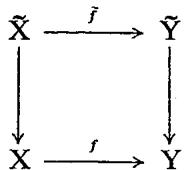
\includegraphics[keepaspectratio]{images/part001_3e847d2c.jpg}}

，并且与群 \(\{\pm1\}\) 的作用相容。

若 \(\tilde{f}\) 是 f 的一个定向，且 \(\eta\) 是 Y 的一个定向，则存在唯一一个 X 的定向 \(\xi\)，使得图表

\pandocbounded{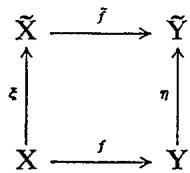
\includegraphics[keepaspectratio]{images/part001_a1f56317.jpg}}

可交换。称 \(\xi\) 由 \(\eta\) 通过 \(f\) 关联得到。

例子

\begin{enumerate}
\def\labelenumi{\alph{enumi})}
\item
  若 Y 退化为一点，则 f 的一个定向等价于 X 的一个定向。
\item
  设 \(f\) 是 étale 的。对于每个 \(x \in X\)，映射 \(\mathrm{T}_{x}(f)\) 是从 \(\mathrm{T}_{x}(\mathrm{X})\) 到 \(\mathrm{T}_{f(x)}(\mathrm{Y})\) 的同构，并通过结构转移定义一个双射
\end{enumerate}

\[
\tilde {f} _ {x}: \mathrm{Or} (\mathrm{T} _ {x} (\mathrm{X})) \rightarrow \mathrm{Or} (\mathrm{T} _ {f (x)} (\mathrm{Y})).
\]

族 \(\tilde{f}_{x}\) 定义了一个态射 \(\tilde{f}\colon\tilde{\mathbf{X}}\to\tilde{\mathbf{Y}}\)，它是 \(f\) 的一个定向，称为典范定向。

\begin{enumerate}
\def\labelenumi{\alph{enumi})}
\setcounter{enumi}{2}
\tightlist
\item
  更一般地，设 \(f\) 是浸没，并令 \(\alpha\) 为丛 T(X/Y) 的一个定向（8.1.3）。设 \(x\in X\)，且 \(\xi\) 是 \(\mathrm{T}_{x}(\mathrm{X}/\mathrm{Y})\) 的一个定向。置 \(y=f(x)\)；我们有正合序列（8.1.3）
\end{enumerate}

\[
0 \rightarrow \mathrm{T} _ {x} (\mathrm{X} / \mathrm{Y}) \rightarrow \mathrm{T} _ {x} (\mathrm{X}) \xrightarrow {\mathrm{T} _ {x} (f)} \mathrm{T} _ {y} (\mathrm{Y}) \rightarrow 0
\]

因而存在唯一一个定向 \(\tilde{f}_{\alpha}(\xi)\)，它是 \(\mathrm{T}_{y}(\mathrm{Y})\) 的定向，使得 \(\xi = \tilde{f}_{\alpha}(\xi)\alpha(x)\)（10.2.1）。映射 \(\tilde{f}_{\alpha}\colon \tilde{\mathrm{X}}\to \tilde{\mathrm{Y}}\) 是 \(f\) 的一个定向，称为与 \(\alpha\) 关联的定向。映射 \(\alpha \mapsto \tilde{f}_{\alpha}\) 是从 \(\mathrm{T}(\mathrm{X}/\mathrm{Y})\) 的定向集合到 \(f\) 的定向集合的双射。

\begin{enumerate}
\def\labelenumi{\alph{enumi})}
\setcounter{enumi}{3}
\tightlist
\item
  若 \(f: X \to Y\) 是浸入，则 \(f\) 的定向与相对于 \(f\) 的法丛的定向相对应。
\end{enumerate}

10.2.6（“乘积的定向”）。设 \(\mathbf{X}_1\)（相应地 \(\mathbf{X}_2\)）是局部有限维流形，且 \(\xi_1\)（相应地 \(\xi_2\)）是 \(\mathbf{X}_1\)（相应地 \(\mathbf{X}_2\)）的一个定向。令 \(\mathbf{X} = \mathbf{X}_1 \times \mathbf{X}_2\)。映射 \((x_1, x_2) \mapsto \xi_1(x_1)\xi_2(x_2)\)（10.2.1）是 \(\mathbf{X}_1 \times \mathbf{X}_2\) 的一个定向，称为定向 \(\xi_1\) 与 \(\xi_2\) 的乘积，记作 \(\xi_1\xi_2\) 或 \(\xi_1 \otimes \xi_2\)。

设 \(X_{i}\)（i = 1, 2）是维数为 \(n_{i}\) 的纯流形。典范同构 \(X_{1} \times X_{2} \to X_{2} \times X_{1}\) 将 \(\xi_{1} \otimes \xi_{2}\) 变为 \(\xi_{2} \otimes \xi_{1}\)（相应地变为 \(-\xi_{2} \otimes \xi_{1}\)）；若某个 \(n_{i}\) 为偶数（相应地，若 \(n_{1}\) 与 \(n_{2}\) 都为奇数）。

10.2.7（“复数情形”）。设 F 是有限维复向量空间，\(F_{R}\) 是其底层实向量空间。设 \(\{e_{1},\ldots,e_{m}\}\) 是 F 的一个基；则 \(\{e_{1},ie_{1},e_{2},ie_{2},\ldots,e_{m},ie_{m}\}\) 是 \(F_{R}\) 的一个基，而由 2m-向量定义的 \(F_{R}\) 的定向

\[
e _ {1} \wedge i e _ {1} \wedge e _ {2} \wedge i e _ {2} \wedge \dots \wedge e _ {m} \wedge i e _ {m}
\]

与 F 的基 \(\{e_{1},\ldots,e_{m}\}\) 的选取无关；这称为由给定复结构定义的 \(F_{R}\) 的定向。若 F 是两个子空间 G 与 H 的直和，则 \(F_{R}=G_{R}\oplus H_{R}\) 的定向是 \(G_{R}\) 与 \(H_{R}\) 的定向的乘积。

设 X 是一个局部有限维实流形，配备一个几乎复结构（8.8.3）。对每个 \(x \in X\)，令 \(\xi(x)\) 为其复结构定义的 \(\mathrm{T}_{x}(\mathrm{X})\) 的定向。映射 \(x \mapsto \xi(x)\) 是 X 的一个定向，称为由几乎复结构定义的定向。特别地，对于一个局部有限维复解析流形 \(X^{c}\) 的底层实解析流形 X，我们赋予它由相应几乎复结构定义的定向（8.8.6）。若把 X 上给定的复解析流形结构替换为其共轭结构（5.4.12.b)），则此定向乘以函数 \(x \mapsto (-1)^{\dim_{x} X^{c}}\)。

10.2.8. 例子

\begin{enumerate}
\def\labelenumi{\alph{enumi})}
\tightlist
\item
  设 E 是有限维实向量空间。由 E 定义的实解析流形（5.2.2）是可定向的。更确切地说，映射 \(\xi \mapsto \xi(0)\) 是从该流形的定向集合到 Or(E) 上的双射。
\end{enumerate}

特别地，流形 \(R^{n}\) 具有一个典范定向 \(\xi^{n}\)，它由半直线 \(R_{+}e_{1}\wedge\cdots\wedge e_{n}\)（属于 \(\mathrm{Or}(\mathbf{R}^{n})\)）定义。

\begin{enumerate}
\def\labelenumi{\alph{enumi})}
\setcounter{enumi}{1}
\item
  设 X 是中心为 0、半径为 \(\rho\) 的 \(\mathbf{R}^n\) 中的球面；它是 \(\mathbf{R}^n\) 的子流形。对每个 \(x \in \mathbf{X}\)，空间 \(\mathbf{T}_x(\mathbf{R}^n) = \mathbf{R}^n\) 是直线 \(\mathbf{R}x\) 与超平面 \(\mathbf{T}_x(\mathbf{X})\) 的直和。令 \(\eta_x\) 为定向 \(\mathbf{R}_+x\) 的直线 \(\mathbf{R}x\)（“向外法向”），并令 \(\xi_x\) 为 \(\mathbf{T}_x(\mathbf{X})\) 的唯一一个定向，使得 \(\eta_x\) 与 \(\xi_x\) 的乘积是定向 \(\xi^n\) 的 \(\mathbf{R}^n\)。映射 \(x \mapsto \xi_x\) 是 \(\mathbf{X}\) 的一个定向，称为典范定向。
\item
  设 X 是一个连通流形，G 是在 X 上适当地且自由地作用的离散群。X/G 可定向的充要条件是 X 可定向且 G 在 X 的定向集合上的作用是平凡的。
\item
  实射影空间 \(\mathbf{P}_{n-1}(\mathbf{R})\) 可与球面 \(S_{n-1}\) 在群 \(\{\pm1\}\) 通过 \(x\mapsto\pm x\) 的作用下的商等同；当 n 为偶数时它可定向，当 n 为奇数时它不可定向。
\item
  每个李群被连通李子群取商所得的空间都是可定向的。
\end{enumerate}

